\section{Vurdering}
På bagrund af graferne i sektion \ref{ch4_design} kan det vurderes, at det designede FIR-filter til en vis grad formår at filtrere frekvensen $\omega_2=\frac{\pi}{2}$ fra det samplede signal $s[n]$ som ønsket ved anvendelse af orden $M=62$ eller derover. \\
Figur \ref{fig:filter_rekt} illustrerer dog, at de opstillede specifikationer kun til en vis grad overholdes ved en orden på henholdsvis 62 og 126 og anvendelse af det rektangulære vindue. Det ses tydeligt, at transitionsbåndet bliver smallere og at stopbåndet flader ud jo højere orden der anvendes. De ripples, der forekommer i pasbåndet formindskes også, når ordenen øges. Dog forsvinder de ikke, da det er det rektangulære vindue, der anvendes, og amplituderesponsen er ikke 0 i stopbåndet, hvormed signalet ikke filteres optimalt. Herunder optimeres filteret ved at anvende Hamming-vinduet.

\section{Optimering}
Forsøg har vist, at der opnås en god filtrering ved hjælp af Hamming-vinduet med $M=126$, hvormed frekvensen $\omega_2 = \pi/2$ i udstrakt grad filtreres fra uden at påvirke de øvrige frekvenser. Dette resultat ses på figur \ref{fig:resultat}, der henholdsvis viser frekvensspektret, hvor frekvensen $\omega_2 \approx 1.57$ ikke fremgår, og en sammenligning mellem det ideelle filtrerede signal og det filtrerede signal. Af sidstnævnte fremgår det, at de to signaler ligger oveni hinanden med enkelte afvigelser.
\begin{figure}[H]
\begin{minipage}{0.49\textwidth}
\centering
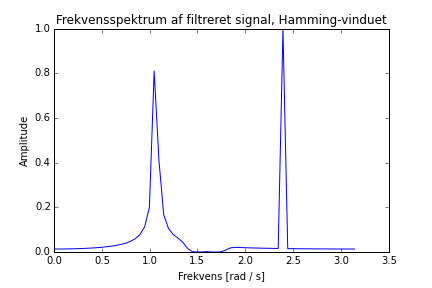
\includegraphics[width=\textwidth]{figures/Filter/freq_filt_signal_Hamming.png}
\end{minipage}
\begin{minipage}{0.49\textwidth}
\centering
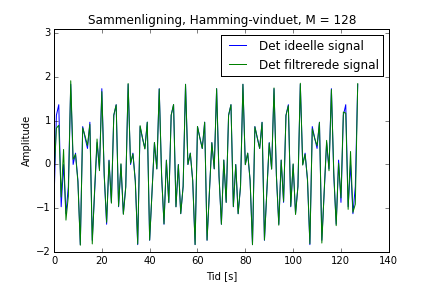
\includegraphics[width=\textwidth]{figures/Filter/signal_compare_Hamming.png}
\end{minipage}
\caption{Frekvensspektrum for det filtrerede signal under anvendelse af filter af orden $M=128$ (venstre) og sammenligning af det filtrerede signal og det ønskede signal (højre).}
\label{fig:resultat}
\end{figure}

Amplituderesponser for Hamming-vinduet med $M = 62$ og $M = 126$ ses desuden på figur \ref{fig:amplituderespons_Hamming} i bilag \ref{app2}. Af disse figurer fremgår det, at et filter med Hamming-vinduet med $M = 126$ er tæt på den ideelle amplituderespons.

\section{Samlet konklusion}
I dette miniprojekt er et signal indeholdende 3 sinus-komponenter blevet genereret og samplet, hvorefter det er blevet analyseret for dets frekvensmæssige indhold ved hjælp af en implementering af DFT'en i form af en FFT-algoritme. Afslutningsvis er signalet blevet filtreret ved hjælp af et båndstopfilter med endelig impulsrespons, som i vid udstrækning har formået at eliminere frekvensen på $\pi/2$ uden at påvirke de øvrige de øvrige frekvenser som ønsket. Resultatet af denne filtrering ses på figur \ref{fig:resultat}.